\subsection{InternVL3-9B 跨骨干验证}
\label{app:internvl}

图~\ref{fig:internvl_trajectory}展示 InternVL3-9B 在 VQA-RAD 与 MIMIC-CXR 上的学习轨迹。两项任务分别训练独立模型，通过 LLaMA-Factory~\citep{zheng2024llamafactory}进行全参数监督微调，每轮从上一轮权重继续训练。曲线包含基线及全部八个已完成训练轮次。

VQA-RAD 准确率由56.98\%提高至第8轮的77.38\%，增加20.40个百分点，并在第6轮达到最高值78.71\%。MIMIC-CXR 的 RaTEScore 由50.55提高至63.83，增加13.28分，第4轮达到最高值65.34。两条轨迹在不同阶段达到峰值，最终轮次仍保留较大的性能增益。

\begin{figure}[H]
\centering
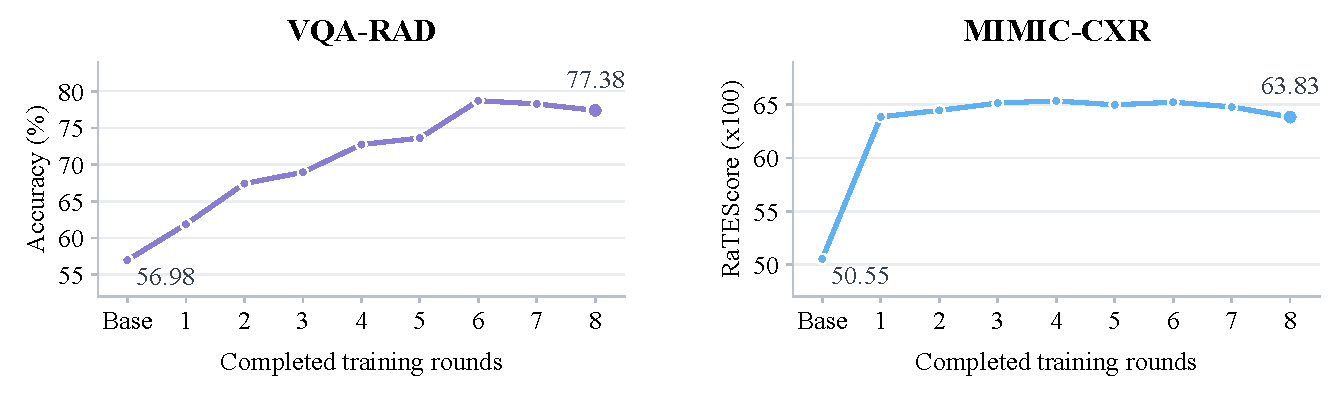
\includegraphics[width=\linewidth]{figures/internvl_trajectory.pdf}
\caption{InternVL3-9B 的学习轨迹。左：VQA-RAD 准确率（\%）；右：MIMIC-CXR RaTEScore，乘以100展示。两个面板对应分别训练的任务专用模型。Base 表示初始模型，1--8表示已完成训练轮次；仅标注基线与最后一轮数值。}
\label{fig:internvl_trajectory}
\end{figure}
